\begin{figure}[H]
    \centering
    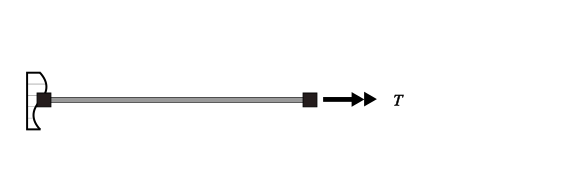
\includegraphics[width=0.9\linewidth]{Examples/frame-0021/img/frame-0021.png}
    \caption{Model for Example~\ref{sec:frame-0021}.}
    \label{fig:0021}
\end{figure}

\subparagraph{Context}
This example investigates non-uniform torsional warping. 
The analytic solution \eqref{eq:0028-gen-rot} to the beam governing equations (Box~\ref{box:exact-shear-svq}) is used as reference. 


A similar example was considered by \cite{lecorvec2012nonlinear}, where 16 warping degrees of freedom were required. 
Here only one warping degree of freedom is used. Excellent agreement with the analytic solution is obtained using both the \ForceFrame{} and \ExactFrame{} elements.


\begin{figure}[H]
    \centering
    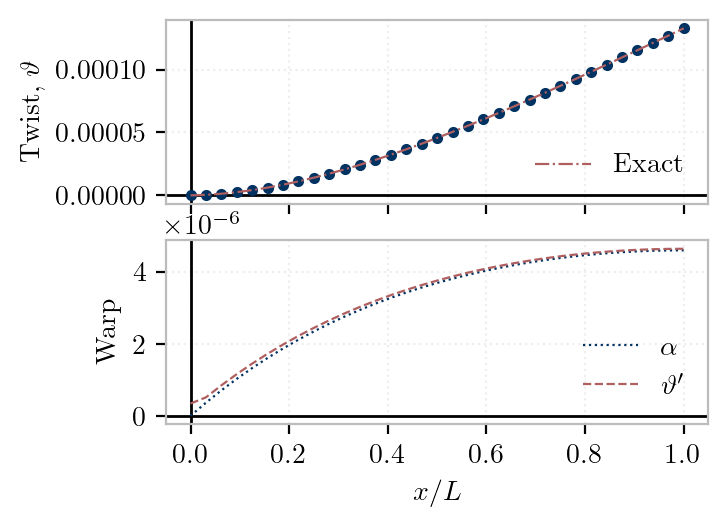
\includegraphics[width=0.46\linewidth]{Examples/frame-0021/img/Force-Shear-w-b-kinematics.png}
    % 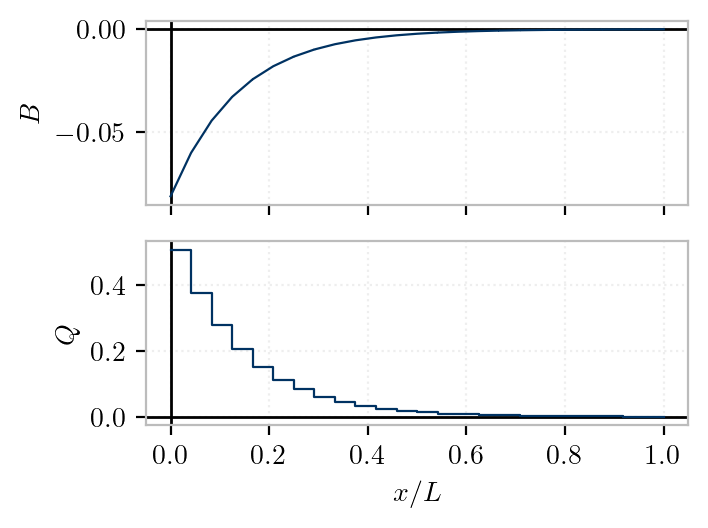
\includegraphics[width=0.45\linewidth]{Examples/frame-0021/img/e0011-resultants-b.png}
    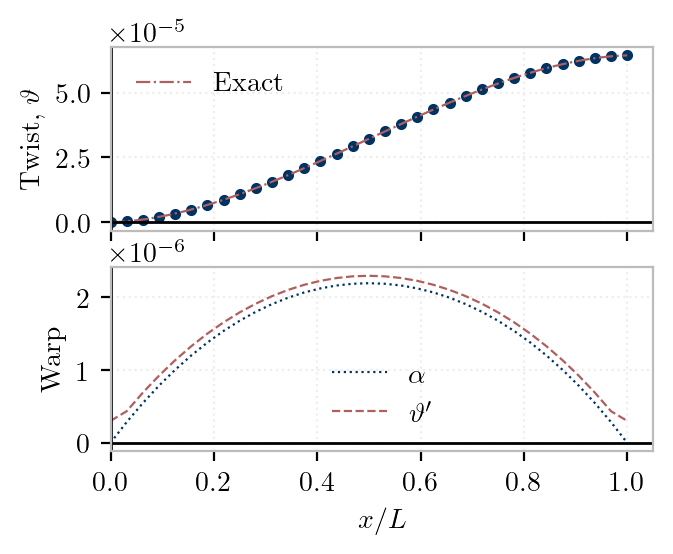
\includegraphics[width=0.46\linewidth]{Examples/frame-0021/img/Force-Shear-w-c-kinematics.png}
    \caption{Warping amplitude \(\alpha\) and twist \(\vartheta\) for Example~\ref{sec:frame-0021}.}
    \label{fig:0021-results}
\end{figure}


\paragraph{Case C: Fixed-Fixed}
Warping is prevented at both sides of a beam furnishing the 1,2/2,4 boundary conditions
$$
\begin{aligned}
\vartheta(0) &= 0 \\ 
\alpha(0) &= 0 \\
\,
\end{aligned}
\qquad\text{ and }\qquad 
\begin{aligned}
\\
\alpha(L) &= 0 \\
\mathrm{R}[\vartheta(L)] &= -\TwistRxn
\end{aligned}
$$
where $\mathrm{R}[\vartheta] = \lambda^2 \vartheta' - \vartheta'''$ is the Robin boundary operator.
% or:
% $$
% \begin{aligned}
% & \left.\vartheta\right|_{x=0}=\vartheta_i,\quad \left.\vartheta' \right|_{x=0}=0 \\
% & \left.\vartheta\right|_{x=L}=\vartheta_j,\quad \left.\vartheta' \right|_{x=L}=0
% \end{aligned}
% $$
%

% From \cite{chen2008theory}:
\begin{equation}
\begin{aligned}
C_1& =-C_2=\frac{1 - \cosh \lambda L}{\sinh \lambda L} \\
C_3& =-1 %\frac{1}{2}
\end{aligned}
\end{equation}


\begin{figure}[H]
    \centering
    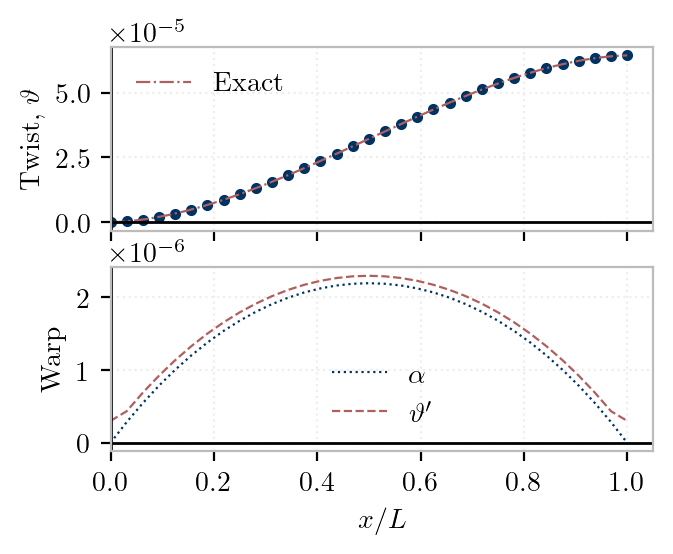
\includegraphics[width=0.48\linewidth]{Examples/frame-0021/img/Force-Shear-w-c-kinematics.png}
    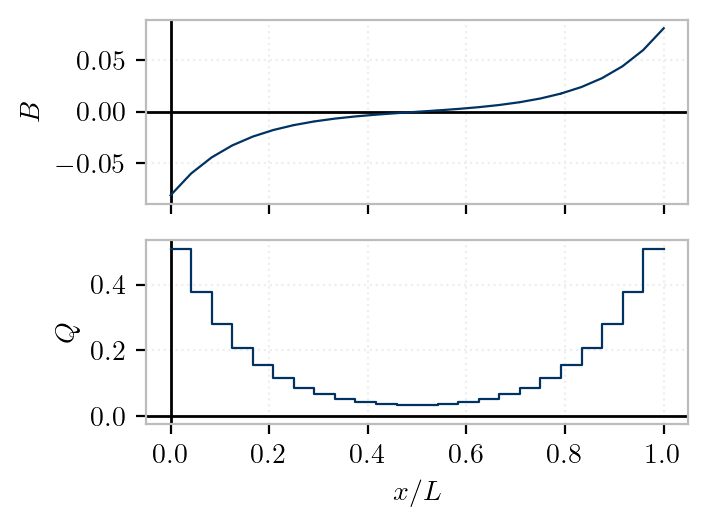
\includegraphics[width=0.48\linewidth]{Examples/frame-0021/img/e0011-resultants-c.png}
    \caption{Warping amplitude \(\alpha\) and twist \(\vartheta\) for Example~\ref{sec:frame-0021} case C.}
    \label{fig:0021c-kinematics}
\end{figure}



\iffalse
\subsubsection{Distributed loading}

Recall the differential equation for a prismatic shaft of length $L$:
$$
E \Jw \vartheta^{\mathrm{iv}} - \TwistRigidity \vartheta'' = m_x
$$
where, $G \Jo$ is the torsion stiffness, $E \Jw$ is the warping stiffness and $m_x$ is a distributed torsion moment along the beam. 
In standard form:
$$
\vartheta^{\mathrm{iv}} - \lambda^2 \vartheta'' = m_x,
\quad 
\lambda \triangleq \sqrt{\frac{GJ}{\eta E\Jw}}
$$

\begin{equation}
\vartheta=C_4+C_5 z+C_6 \cosh \lambda z+C_7 \sinh \lambda z-\frac{m_z}{2 \lambda^2 E I_{t r}} x^2
\end{equation}


\subparagraph{Case B: }
The element stiffness matrix is
\begin{equation}
\begin{aligned}
\begin{pmatrix}
T_i \\
T_j
\end{pmatrix}
&=\frac{\beta\left(1+e^{2 \beta}\right)}{\beta+1+(\beta-1) e^{2 \beta}}
\frac{G J}{L}
\left[\begin{array}{cc}
 1 & -1 \\
-1 &  1
\end{array}\right]
\begin{pmatrix}
\vartheta_i \\
\vartheta_j
\end{pmatrix}\\
&+\frac{m_x}{\beta\left(\beta+1+(\beta-1) e^{2 \beta}\right)}\left[\begin{array}{c}
-\frac{1}{2}\left(\beta^2-2+4 e^\beta+\left(\beta^2-2\right) e^{2 \beta}\right) L \\
-\frac{1}{2}\left(\beta^2+2 \beta+2-4 e^\beta+\left(\beta^2-2 \beta+2\right) e^{2 \beta}\right) L
\end{array}\right]
\end{aligned}
\end{equation}

\subparagraph{Case C: Fixed-Fixed}
Warping is prevented at both sides of a beam furnishing the boundary conditions
$$
\begin{aligned}
& \left.\vartheta\right|_{x=0}=\vartheta_i,\quad \left.\vartheta' \right|_{x=0}=0 \\
& \left.\vartheta\right|_{x=L}=\vartheta_j,\quad \left.\vartheta' \right|_{x=L}=0
\end{aligned}
$$
%
The solution for a constant distributed torque \(m_x\) is
\begin{equation*}
\begin{aligned}
\vartheta&=\left(\vartheta_j-\vartheta_i\right) \frac{\lambda x+1+\left(\lambda x-1\right) e^\beta-e^{\lambda x}+e^{\beta\left(1-\frac{x}{L}\right)}}{\beta+2+(\beta-2) e^\beta} \\
&+m_x G J \frac{\lambda x+1-\beta \frac{x^2}{L^2}-\left(\lambda x-1-\beta \frac{x^2}{L^2}\right) e^\beta-e^{\lambda x}-e^{\beta\left(1-\frac{x}{L}\right)}}{2 \beta L^2\left(1-e^\beta\right)}
\end{aligned}
\end{equation*}
Using, $T_i=-\left.T\right|_{x=0}, B_i=\left.B\right|_{x=0}, T_j=\left.T\right|_{x=L}$ and $B_2=-\left.B\right|_{x=L}$ the element stiffness matrix is

$$
\begin{pmatrix}
T_i \\ T_j
\end{pmatrix}
=\frac{\beta\left(1+e^\beta\right)}{\beta+2+(\beta-2) e^\beta}
\frac{G J}{L}
\begin{bmatrix}
 1 & -1 \\
-1 &  1
\end{bmatrix}
\begin{pmatrix}
\vartheta_i \\ \vartheta_j
\end{pmatrix}
+ m_x \begin{pmatrix}
-\frac{1}{2} L \\
-\frac{1}{2} L
\end{pmatrix}
$$
%
The bi-moments at both ends can be expressed in terms of the torsion moment

$$
\begin{aligned}
& B_i=-T \frac{L}{\beta} \tanh \left(\frac{1}{2} \beta\right)+m_x \frac{L^2}{\beta^2} \frac{2 \beta e^\beta+1-e^{2 \beta}}{1-e^{2 \beta}} \\
& B_j=-T \frac{L}{\beta} \tanh \left(\frac{1}{2} \beta\right)-m_x \frac{L^2}{\beta^2} \frac{2 \beta e^\beta+1-e^{2 \beta}}{1-e^{2 \beta}}
\end{aligned}
$$
\fi